\documentclass[11pt,a4paper]{article}

% Standard academic packages
\usepackage[utf8]{inputenc}
\usepackage{amsmath, amssymb, amsfonts}
\usepackage{graphicx}
\usepackage{booktabs}
\usepackage{multirow}
\usepackage{tikz}
\usepackage{pgfplots}
\pgfplotsset{compat=1.18}
\usetikzlibrary{shapes.geometric, arrows.meta, positioning, fit, calc, backgrounds}
\usepackage{hyperref}
\usepackage[margin=1in]{geometry}
\usepackage{caption}
\usepackage{cite}
\usepackage{xcolor}
\usepackage{enumitem}
\usepackage{algorithm}
\usepackage{algpseudocode}
\usepackage{mathrsfs}

% Polishing packages
\usepackage{microtype}
\usepackage{titlesec}
\usepackage[most]{tcolorbox}
\usepackage{fancyhdr}

% Fix for fancyhdr warnings
\setlength{\headheight}{24pt}
\addtolength{\topmargin}{-12pt}

% Define Custom Colors based on the polished theme
\definecolor{PreprintBlue}{RGB}{34, 84, 142}
\definecolor{AbstractBg}{RGB}{245, 248, 252}
\definecolor{AbstractBorder}{RGB}{176, 200, 230}
\definecolor{HighlightGreen}{RGB}{46, 139, 87}
\definecolor{AlertRed}{RGB}{178, 34, 34}

% Customizing hyperref colors
\hypersetup{
    colorlinks=true,
    linkcolor=PreprintBlue,
    filecolor=magenta,
    urlcolor=PreprintBlue,
    citecolor=PreprintBlue,
}

% Formatting Headers with titlesec
\titleformat{\section}
  {\Large\bfseries\color{PreprintBlue}}
  {\thesection}{1em}{}
\titleformat{\subsection}
  {\large\bfseries\color{PreprintBlue}}
  {\thesubsection}{1em}{}
\titleformat{\subsubsection}
  {\normalsize\bfseries\color{PreprintBlue}}
  {\thesubsubsection}{1em}{}

% Customizing Page Headers
\pagestyle{fancy}
\fancyhf{}
\fancyhead[L]{\color{gray}\small \textit{Heterogeneous Compute Cascades}}
\fancyhead[R]{\color{gray}\small Preprint -- April 2026}
\fancyfoot[C]{\thepage}
\renewcommand{\headrulewidth}{0.4pt}
\renewcommand{\headrule}{\hbox to\headwidth{\color{gray}\leaders\hrule height \headrulewidth\hfill}}

% Title, Author, Date
\makeatletter
\renewcommand{\maketitle}{
    \bgroup\setlength{\parindent}{0pt}
    \begin{center}
        \vspace*{1em}
        {\LARGE \bfseries \color{PreprintBlue} Heterogeneous Compute Cascades: \\[0.3em] A Cost-Effective Architectural Solution for \\[0.3em] 370B-Parameter MoE Inference on Edge Clusters \par}
        \vspace{1.5em}
        {\large Julian Beltran \par}
        \vspace{0.5em}
        {\color{gray} Independent Researcher \\ \texttt{julian@dinference.com} \par}
        \vspace{1em}
        {\color{gray} \textit{Draft Prepared for Peer Review} -- April 2026 \par}
    \end{center}
    \egroup
    \vspace{1em}
}
\makeatother

\begin{document}

\maketitle

\begin{center}
\begin{tcolorbox}[
    colback=AbstractBg,
    colframe=AbstractBorder,
    boxrule=0.5pt,
    arc=4pt,
    left=10pt,
    right=10pt,
    top=10pt,
    bottom=10pt
]
\textbf{Abstract.} The democratization of frontier artificial intelligence is fundamentally blocked by the capital expenditure (CAPEX) and thermodynamic footprint required to host models exceeding 100 billion parameters. While a dual-node 16-Core Ryzen APU cluster provides a 256 GB unified memory pool---structurally capable of holding a 744B-parameter GLM-5.1 MoE (380B after REAP pruning)---traditional distributed execution frameworks over consumer USB4 bridges suffer from catastrophic network pipeline bubbles driven by TCP/IP OS kernel latency.

We introduce the \textit{Heterogeneous Compute Cascade} (HCC), a software architecture designed to convert this hardware limitation into a strategic advantage. Rather than treating heterogeneous IP blocks (CPU, iGPU, NPU) as a uniform compute pool, HCC enforces strict silicon-to-task affinity. The proposed architecture assigns context compression and draft generation to the NPU, with a projected activation reduction above 80\% and speculative latency hiding across USB4. These accelerator paths are design targets: the current runtime validates a stop-and-wait typed protocol in simulation, while physical NPU compression and overlap remain unimplemented.

Furthermore, to ensure the KV cache does not exhaust unified memory during long-context execution, the architecture proposes 3-bit TurboQuant KV compression via Walsh-Hadamard rotations. The target software stack specifies kernel-level DMA-BUF descriptors to bridge the iGPU (via MIGraphX) and NPU (via Vitis AI); the present prototype uses framed TCP plus a host-memory \texttt{memfd}/\texttt{mmap} scaffold and does not yet implement cross-driver zero-copy. Our analytical model projects a $\sim$3$\times$ improvement in Time-to-First-Token (TTFT) and a 2.35$\times$ multiplier on decode throughput relative to na\"ive RPC bridging. Theoretical analysis indicates a hardware cost of \$20.31 per GB of addressable memory---representing a projected 92\% cost reduction and 96\% power reduction versus a turnkey DGX A100 deployment. This work demonstrates, through formal mathematical analysis, that intelligent orchestration rather than raw interconnect bandwidth is the key architectural principle for enabling massive-scale AI inference at the edge.
\end{tcolorbox}
\end{center}

\vspace{0.5cm}
\noindent\textbf{Keywords:} distributed inference, latency hiding, AMD 16-Core Ryzen APU, XDNA 2, TurboQuant, ONNX Runtime, Mixture of Experts (MoE), TCO optimization, edge computing, speculative decoding

\newpage
\tableofcontents
\vspace{1em}

\section{Introduction: The Hardware Inaccessibility Crisis}

\begin{tcolorbox}[colback=AbstractBg, colframe=AbstractBorder, boxrule=0.3pt, arc=3pt, left=8pt, right=8pt, top=6pt, bottom=6pt]
\small\textbf{Paper Scope.} This document constitutes an \textit{architectural feasibility study} and formal mathematical analysis. It is not a product datasheet, benchmark report, or empirical evaluation. All performance figures are derived from roofline models, theoretical bounds, and published hardware specifications. Where numerical projections are presented, they represent theoretical upper bounds under ideal conditions. The experimental validation roadmap is described in Section~\ref{sec:validation}.
\end{tcolorbox}
\vspace{0.5em}

The relentless scaling laws governing Large Language Models (LLMs) have precipitated a crisis in hardware accessibility. As the frontier of intelligence pushes past 100 billion parameters (e.g., Llama-3-400B, Grok-1.5, GLM-5.1), the memory required to simply load model weights often exceeds 200 GB. Single consumer graphics processing units (GPUs) currently peak at 24 GB to 48 GB of Video RAM (VRAM). To execute these models locally, researchers and enterprises are forced into traditional data center scaling paradigms---utilizing specialized server-grade interconnects such as NVIDIA's NVLink across multi-GPU arrays (e.g., an $8\times$ H100 SXM node).

This legacy approach relies on brute-force parallelism and incurs a prohibitive Total Cost of Ownership (TCO). A single high-bandwidth cluster demands upwards of \$80,000 in capital expenditure, requires massive thermal dissipation (often exceeding 3500W per node), and restricts frontier AI research to heavily funded, centralized institutions. The push toward Sovereign AI requires a localized alternative.

The 16-Core Ryzen APU architecture represents a pivotal paradigm shift for high-performance edge computing. By combining a 40-CU RDNA 3.5 integrated GPU (iGPU), an advanced XDNA 2 Neural Processing Unit (NPU) capable of 50 Tera Operations Per Second (TOPS), and a 256-bit memory bus supporting up to 128 GB of LPDDR5x-8000 unified memory per System-on-Chip (SoC) \cite{ryzen16core}, the platform fundamentally changes the economics of VRAM capacity.

By networking two such systems via a consumer 40 Gbps USB4 bridge, a decentralized cluster with 256 GB of aggregate memory can be assembled for approximately \$5,200 (\$2,600 per node). Yet, physical capacity does not equal performant execution. Standard software frameworks like \texttt{llama.cpp} over a USB4 TCP/IP bridge yield crippled performance due to the inherent latency of transmitting massive hidden-state activation tensors across an OS-managed network stack \cite{geerling2025, llama_rpc}.

To address this, we propose the \textbf{Heterogeneous Compute Cascade (HCC)}---a specialized architectural solution designed to pair specific computational tasks (prefill, decode, KV caching) with the silicon block (NPU, iGPU, CPU) best suited for each mathematical profile. This paper presents the formal analysis demonstrating how HCC is architected to accelerate token generation, reduce operating power, and provide a compelling economic advantage.

\section{Microarchitectural Profiling of AMD 16-Core Ryzen APUs}

To successfully orchestrate a massive MoE across edge nodes, we must mathematically map the capabilities of the underlying silicon. The AMD 16-Core Ryzen APU deviates significantly from traditional CPU-GPU desktop pairings.

\subsection{The Memory Subsystem: LPDDR5x and MALL Cache}
Integrated GPUs inherently suffer from bandwidth starvation because they share a memory bus with the CPU. The 16-Core Ryzen APU mitigates this by implementing a desktop-class 256-bit memory interface. When paired with LPDDR5x operating at 8000 MT/s, the theoretical peak memory bandwidth reaches $256 \text{ GB/s}$.

Crucially, the architecture incorporates a dedicated \textbf{32 MB MALL (Memory Attached Last Level) cache}, synonymous with AMD's Infinity Cache \cite{ryzen16core}. Placed on the main Graphics Compute Die (GCD), the MALL cache acts as a high-speed buffer. While theoretical bandwidth is 256 GB/s, published measurements indicate an effective, sustained yield of approximately $212 \text{ GB/s}$ when the MALL cache is utilized to capture repeated attention head memory reads.

\subsection{XDNA 2 and AIE-ML v2 Spatial Dataflow}
The most unexploited asset in edge inference is the NPU. The XDNA 2 architecture introduces the \textbf{AIE-ML v2} (AI Engine for Machine Learning, version 2). Unlike traditional CPUs or GPUs that rely on rigid temporal cache hierarchies, XDNA 2 employs a \textbf{spatial dataflow architecture} \cite{xdna2}.

It consists of a 2D grid of 32 independent compute tiles. Each tile houses a Very Long Instruction Word (VLIW) SIMD vector processor, a scalar RISC core, and 64 KB of local SRAM. Interspersed in the array are 512 KB shared memory tiles. In a spatial dataflow model, data ``flows'' directly from one tile's SRAM to the next through a programmable interconnect fabric, bypassing main system DDR memory entirely.

Furthermore, XDNA 2 supports \textbf{Block FP16 (BFP16)}. Standard FP16 retains massive dynamic range but requires 16 bits of bandwidth per value. BFP16 clusters values into blocks, storing individual 8-bit mantissas that share a single 8-bit exponent. This allows the XDNA 2 array to process activations at INT8 hardware speeds while preserving the numerical fidelity required by LLMs.

\section{Background and Formalization of MoE Architectures}

\subsection{Distributed Edge Inference and Interconnect Topologies}
Apple Silicon clusters (e.g., Mac Studio arrays) rely on the proprietary \textit{UltraFusion} interposer, delivering 2.5 TB/s of bidirectional bandwidth \cite{apple_unified}. However, these systems scale poorly beyond a single physical node without exorbitant cost. Conversely, clustering consumer x86 hardware relies on external peripheral bridges such as USB4. While USB4 advertises 40 Gbps ($\sim$5 GB/s) of bandwidth, pipeline-parallel TCP execution can incur substantial software latency from RPC serialization and network-stack traversal \cite{llama_rpc}. Section 5.1 therefore treats 17 $\mu$s as a tuned model input that must be reproduced on the target pair.

\subsection{Mixture of Experts and Router-Weighted Expert Activation Pruning}
Mixture of Experts (MoE) architectures decouple the total parameter count of a network from its active computational cost. For a given input token $x$, the output $y$ is computed as the weighted sum of the selected experts:
\begin{equation}
    y = \sum_{i=1}^{E} G(x)_i \cdot E_i(x)
\end{equation}
where $E$ is the total number of experts, $E_i(x)$ is the expert output, and $G(x)_i$ is the gating probability. To enforce sparsity, a noisy Top-$K$ routing mechanism is employed:
\begin{equation}
    G(x) = \text{Softmax}\left(\text{Top}_K(x \cdot W_g + \epsilon \cdot \text{Softplus}(x \cdot W_{\text{noise}}))\right)
\end{equation}

We apply Router-Weighted Expert Activation Pruning (REAP) \cite{reap} (Cerebras Research, arXiv 2025; validated on GLM, Qwen, and DeepSeek model families) to the open-weight GLM-5.1 model \cite{glm5} ($\sim$744B parameters, 256 routed experts, $L=78$ layers, $H=6144$). GLM-5.1 employs \textbf{Multi-head Latent Attention (MLA)} with compressed KV projections ($\text{kv\_lora\_rank}=512$, $\text{qk\_rope\_head\_dim}=64$) and \textbf{DeepSeek Sparse Attention (DSA)} for efficient long-context handling up to 200K tokens. MLA stores only 576 values per token per layer in the KV cache---an order of magnitude smaller than standard GQA---which is a key enabler of the HCC memory budget.

REAP scores each expert as $\text{mean}(w_{\text{router}} \cdot \|e_{\text{out}}\|_2)$ and removes the lowest-scoring half. We quantize the pruned checkpoint using \textbf{Unsloth Dynamic 2.0} quantization \cite{unsloth}, which adaptively preserves quality-critical layers at higher precision while aggressively compressing redundant layers. GLM-5.1 (released April 9, 2026) produces slightly smaller Unsloth quantizations than GLM-5 due to improved weight distributions---e.g., UD-IQ2\_M is 236 GB for GLM-5.1 vs.\ 255 GB for GLM-5---making it the preferred target for memory-constrained deployments.

The resulting \textbf{GLM-5.1-REAP-50} comprises $\sim$380B total parameters across $E=128$ remaining experts, with $\sim$40B active per forward pass ($K=8$). At UD-Q3\_K\_M, the REAP-50 checkpoint occupies $\sim$161 GB, fitting comfortably within a dual-node 256 GB cluster with ample headroom for the KV cache and OS. At the more aggressive UD-IQ2\_M, the checkpoint shrinks to $\sim$121 GB---small enough to fit on a \textit{single} 128 GB node, eliminating the dual-node requirement entirely for latency-insensitive deployments. Crucially, the original REAP evaluation demonstrates that pruning 50\% of experts based on router-weight-scaled activation norms incurs a negligible $<$1.5 point penalty on zero-shot MMLU and maintains coding proficiency on HumanEval, confirming that this aggressive compression preserves frontier-class reasoning capabilities rather than producing a fundamentally degraded model.

\section{Related Work}

\textbf{Distributed edge inference.} Petals \cite{petals} distributes model layers across volunteer nodes over the Internet. The \texttt{llama.cpp} RPC backend \cite{llama_rpc} implements pipeline parallelism over TCP but suffers catastrophic pipeline bubbles on USB4 bridges. HCC differs by exploiting on-die heterogeneous silicon (NPU, iGPU) to \textit{hide} interconnect latency rather than merely tolerating it.

\textbf{Speculative decoding.} Leviathan et al.\ \cite{spec_decode} showed that a small draft model can propose tokens verified in parallel by the target model. HCC repurposes this paradigm for \textit{latency amortization}: each speculative batch amortizes the USB4 network crossing cost over $\mathbb{E}[k]$ accepted tokens.

\textbf{MoE compression.} REAP \cite{reap} prunes entire experts by router-weight-scaled activation norms. DeepSeek-V3 \cite{deepseek} employs expert parallelism with auxiliary-loss-free load balancing. HCC builds on REAP-pruned models and additionally compresses the KV cache.

\textbf{KV cache quantization.} QuaRot \cite{quarot} applies Walsh-Hadamard rotations to remove outliers before 4-bit quantization. TurboQuant \cite{turboquant} (Google Research / NYU, arXiv 2025; validated on LongBench-E and Needle-in-a-Haystack at 104K tokens) extends this to near-optimal 3-bit vector quantization with QJL residual correction \cite{qjl} (Zandieh et al., arXiv 2024; open-source implementation at \texttt{github.com/amirzandieh/QJL}). KIVI \cite{kivi} achieves 2-bit KV quantization asymmetrically. HCC mandates TurboQuant-class compression as a structural requirement.

\textbf{Application-layer context reduction.} While HCC addresses the physical interconnect bottleneck at the hardware layer, application-layer frameworks such as Cascaded Signal Refinement (CSR) \cite{csr} address the \textit{logical} context bottleneck. CSR employs a three-layer pipeline---deterministic pre-filtering, small-model LLM screening, and deep analysis---to reduce enterprise compliance corpora by 96.9\% prior to expensive inference, processing 27,020 messages in 98.7 seconds on a consumer GPU using a 4B-parameter model. HCC provides the natural zero-data-transit hardware substrate for such sovereign, multi-layered inference pipelines.

\section{The Interconnect Bottleneck (The Problem)}

To appreciate the HCC solution, we must first formalize the failure mechanics of na\"ive clustering. In a standard pipeline parallel distributed setup, the MoE layers are partitioned sequentially across devices.

We define the network transmission time $T_{\text{comm}}$ with payload $S$, effective bandwidth $B$, protocol overhead $O_{\text{tcp}}$, base latency $L$, and MTU packet size $M$:
\begin{equation}
    T_{\text{comm}} = L + \frac{S}{B} + \left\lceil \frac{S}{M} \right\rceil \cdot O_{\text{tcp}}
\end{equation}

For a model with hidden size $H = 6144$ utilizing FP16 precision:
\begin{itemize}
    \item \textbf{Decode Phase Bubble:} Transmitting a single token's activation requires $1 \times 6144 \times 2 = 12$ KB. Traversing an unoptimized OS TCP/IP stack establishes a latency floor of $\sim$0.5 ms per node crossing \cite{geerling2025} (reduced to $\sim$17 $\mu$s with the kernel tuning described in Section 5.1). Node 2 is idle (a pipeline bubble) while waiting for this transmission.

    \item \textbf{Prefill Phase Bubble:} Transmitting a 100,000-token Retrieval-Augmented Generation (RAG) document requires $100,000 \times 6144 \times 2 \approx 1.23$ GB of data. Utilizing IP-over-Thunderbolt (MTU 9000), effective TCP throughput peaks at approximately 1.25 GB/s.
    \begin{equation}
        T_{\text{stall}} = \frac{1.23 \text{ GB}}{1.25 \text{ GB/s}} + \text{TCP Overhead} \approx 0.984 \text{ seconds}
    \end{equation}
    This dictates a $\sim$1 second pure network stall \textit{per RPC boundary}.
\end{itemize}

\begin{figure}[ht!]
\centering
\begin{tikzpicture}[xscale=0.85]
\draw[->, thick] (0, 0) -- (14, 0) node[right] {\small Time};
\node[anchor=east, font=\small\bfseries] at (0, 2.6) {Node 1};
\fill[PreprintBlue!40] (0.5, 2.3) rectangle (3, 3) node[midway, font=\scriptsize] {Compute L0--38};
\fill[gray!20] (3, 2.3) rectangle (4.5, 3) node[midway, font=\scriptsize] {\textit{Wait}};
\fill[PreprintBlue!40] (4.5, 2.3) rectangle (7, 3) node[midway, font=\scriptsize] {Compute L0--38};
\fill[gray!20] (7, 2.3) rectangle (8.5, 3) node[midway, font=\scriptsize] {\textit{Wait}};
\fill[PreprintBlue!40] (8.5, 2.3) rectangle (11, 3) node[midway, font=\scriptsize] {Compute L0--38};
\draw[thick] (0, 2.2) -- (14, 2.2);
\node[anchor=east, font=\small\bfseries] at (0, 1.2) {Node 2};
\fill[gray!20] (0.5, 0.9) rectangle (3.5, 1.6) node[midway, font=\scriptsize] {\textit{Bubble (idle)}};
\fill[AlertRed!30] (3.5, 0.9) rectangle (4, 1.6);
\fill[PreprintBlue!40] (4, 0.9) rectangle (4.5, 1.6);
\fill[gray!20] (4.5, 0.9) rectangle (7.5, 1.6) node[midway, font=\scriptsize] {\textit{Bubble (idle)}};
\fill[AlertRed!30] (7.5, 0.9) rectangle (8, 1.6);
\fill[PreprintBlue!40] (8, 0.9) rectangle (8.5, 1.6);
\fill[gray!20] (8.5, 0.9) rectangle (11.5, 1.6) node[midway, font=\scriptsize] {\textit{Bubble (idle)}};
\draw[thick] (0, 0.8) -- (14, 0.8);
\draw[->, AlertRed, thick] (3, 2.3) -- (3.5, 1.6);
\draw[->, AlertRed, thick] (7, 2.3) -- (7.5, 1.6);
\end{tikzpicture}
\caption{Pipeline bubble in na\"ive RPC execution. Node~2 idles during Node~1 computation and USB4 transfer, wasting $\sim$50\% of cluster compute. HCC is designed to eliminate this via NPU speculative pre-computation.}
\label{fig:pipeline_bubble}
\end{figure}

\subsection{USB4 Interconnect Reference Parameters}

To ground the analytical model, we use reference parameters for dual USB4 point-to-point (P2P) links between two 16-Core Ryzen APU unified-memory nodes. The values in this section are model inputs retained for reproducibility; they have not been reproduced by the current repository's measurement harness. The intended physical configuration uses native USB4 host-to-host networking tunneled over the Linux \texttt{thunderbolt-net} stack.

\subsubsection{Throughput Assumptions}
The roofline model uses the following single- and dual-link assumptions:

\begin{table}[ht!]
\centering
\caption{USB4 P2P throughput parameters used by the analytical model (not reproduced by the current harness).}
\vspace{0.2cm}
\begin{tabular}{l r r}
\toprule
\textbf{Configuration} & \textbf{Per-Direction} & \textbf{Aggregate} \\
\midrule
Single USB4 link & 11.5 Gbps & $\sim$23 Gbps \\
Dual bonded USB4 links & 22.5 Gbps & $\sim$\textbf{45 Gbps} \\
10 GbE NIC (reference) & 10 Gbps & $\sim$20 Gbps \\
\bottomrule
\end{tabular}
\label{tab:usb4_throughput}
\end{table}

\noindent Dual bonded USB4 achieves approximately \textbf{4.5$\times$} the throughput of a single 10 Gigabit Ethernet link, without requiring any PCIe expansion slots or dedicated network hardware.

\subsubsection{Latency Assumptions}
The latency model uses the following tuned reference values:

\begin{table}[ht!]
\centering
\caption{USB4 P2P round-trip latency parameters used by the analytical model (not reproduced by the current harness).}
\vspace{0.2cm}
\begin{tabular}{l r r r}
\toprule
\textbf{Metric} & \textbf{USB4 P2P (tuned)} & \textbf{10 GbE P2P (tuned)} & \textbf{Improvement} \\
\midrule
Minimum RTT & 14.13 $\mu$s & 16.8 $\mu$s & 16\% \\
Average RTT & 17.35 $\mu$s & 20.7 $\mu$s & 16\% \\
P99 RTT (baseline) & 97 $\mu$s & --- & --- \\
P99 RTT (tuned) & \textbf{27.85 $\mu$s} & --- & 71\% reduction \\
\bottomrule
\end{tabular}
\label{tab:usb4_latency}
\end{table}

\noindent Under these assumptions, raw USB4 network RTT is \textbf{14--28 $\mu$s}, approximately 30$\times$ below the $\sim$0.5 ms per-crossing latency used for an unoptimized \texttt{llama.cpp} RPC comparison. Physical measurements on the target pair remain a validation requirement.

\subsubsection{Kernel-Level Optimizations}
The analytical model assumes a P99 latency reduction from 97 $\mu$s to 27.85 $\mu$s after tuning. The following settings are candidates for physical validation on the target pair; the current repository does not establish their individual or combined effect:
\begin{itemize}[nosep]
    \item \textbf{AMD P-State EPP scheduler:} Replacing legacy C-state disabling with the modern \texttt{amd-pstate} Energy Performance Preference (EPP) scheduler ensures the USB4 controller and NPU tiles remain in a low-latency ready state without compromising the SoC's thermodynamic efficiency---a critical advantage over brute-force \texttt{max\_cstate=1} approaches that waste power.
    \item \textbf{PCIe ASPM disablement:} Disabling Active State Power Management (\texttt{pcie\_aspm=off}) prevents link retraining delays on the Thunderbolt controller.
    \item \textbf{BBR congestion control:} TCP BBR's model-based pacing reduces bufferbloat compared to CUBIC's loss-based approach.
    \item \textbf{Busy-poll sockets:} \texttt{SO\_BUSY\_POLL} with \texttt{napi\_defer\_hard\_irqs} reduces interrupt-to-userspace latency for small RPC payloads.
\end{itemize}

\subsubsection{Implications for LLM Inference}
For the representative $H=6144$ activation exchange analyzed here, each token transfers approximately 12 KB in FP16. At the assumed link capacity, serialization time is small relative to per-call software latency; this motivates HCC's speculative decoding approach, which amortizes crossings over multiple accepted tokens. End-to-end traffic must still be measured on the final sharded runtime.

\subsection{The Single-Node Memory Contention Failure Mode}

Recent community benchmarking (March 2026) has demonstrated that while an 8B model can execute at 43.7 T/s natively on the XDNA 2 NPU \cite{xdna_community}, attempting single-node speculative decoding (NPU draft + iGPU target) yields zero effective speedup. This failure occurs because both accelerators saturate the shared 256-bit LPDDR5x memory bus simultaneously (which community tests cap at a real-world sustained $\sim$215 GB/s), creating catastrophic memory bandwidth contention. As established in recent heterogeneous decoding literature \cite{hetero_spec}, speculative decoding on unified memory platforms cannot succeed if both models fiercely contend for the same physical SoC memory bus. This failure mode is the fundamental motivation for the dual-node HCC architecture.

\section{The HCC Solution: Silicon-to-Task Affinity}

The \textbf{Heterogeneous Compute Cascade (HCC)} is a software orchestration architecture designed to address the interconnect bottleneck by matching specific AI workloads to the silicon blocks best engineered for them.

\subsection{Silicon-to-Task Mathematical Profiling}
We formalize the performance boundaries of the 16-Core Ryzen APU architecture using a Roofline Model. The theoretical compute bound $P$ (in TFLOPS) is defined as $P = \min(P_{\text{peak}}, I \cdot BW_{\text{mem}})$, where $I$ is arithmetic intensity.

\begin{enumerate}
    \item \textbf{Token Generation (Low $I$, High Bandwidth):} Auto-regressive generation has extremely low arithmetic intensity ($I \approx 1$). The node is strictly memory-bound. At 212 GB/s on the RDNA 3.5 iGPU, the theoretical upper bound for decode speed across 40B active parameters (UD-Q3\_K\_M at 0.48 bytes/weight $\approx$ 19.1 GB) is $\sim$11.1 T/s per node.
    \item \textbf{Prompt Prefill (High $I$, Compute Bound):} Prefill operates on large prompt matrices, drastically increasing arithmetic intensity ($I \gg 100$). The XDNA 2 NPU, offering 50 TOPS and specifically designed for high-$I$ tensor contractions, becomes the optimal block.
\end{enumerate}

\noindent Crucially, the HCC architecture solves the single-node memory contention failure described in Section 5.2 through \textbf{physical isolation}. By explicitly mapping the draft model to the NPU on Node~1, and the target MoE execution to the iGPU on Node~2, the workload utilizes \textit{two independent} 256-bit memory buses. The 17 $\mu$s USB4 link acts as the synchronization bridge, allowing the draft model to achieve its full throughput on Node~1's memory without starving the target model's bandwidth on Node~2.

A naive alternative would be to execute the draft model on Node~1's iGPU. However, in our pipeline-parallel topology (Figure 3), Node~1's iGPU is fully saturated executing Layers 0--38 of the target model. Tasking it with draft generation would introduce severe context-switching and memory contention against the main model. The XDNA~2 NPU is the only compute block on Node~1 capable of asynchronous execution without disrupting the main iGPU memory pipeline, making its heterogeneous utilization \textit{structurally mandatory}, not merely a power optimization.

\begin{figure}[ht!]
\centering
\begin{tikzpicture}
\begin{loglogaxis}[
    title={Roofline Model for 16-Core Ryzen APU},
    xlabel={Arithmetic Intensity $I$ (FLOPs/Byte)},
    ylabel={Performance (GFLOPS)},
    domain=0.1:1000,
    grid=both,
    width=0.8\textwidth,
    height=8cm,
    legend pos=south east,
    ymin=10, ymax=100000,
    xmin=0.1, xmax=1000
]
\addplot[thick, PreprintBlue, samples=100] {min(50000, 212 * x)};
\addlegendentry{Hardware Limit (50 TOPS, 212 GB/s)}
% Decode point with callout (avoids overlapping the slope line)
\node[circle,fill=AlertRed,inner sep=2.5pt] at (axis cs:2, 424) {};
\node[anchor=east, font=\small\bfseries] at (axis cs:1.5, 900) {Decode (iGPU)};
\draw[->, thin, gray] (axis cs:1.6, 750) -- (axis cs:1.95, 450);
% Prefill point with callout (avoids overlapping the ceiling)
\node[circle,fill=HighlightGreen,inner sep=2.5pt] at (axis cs:300, 50000) {};
\node[anchor=west, font=\small\bfseries] at (axis cs:400, 25000) {Prefill (NPU)};
\draw[->, thin, gray] (axis cs:380, 28000) -- (axis cs:310, 47000);
\end{loglogaxis}
\end{tikzpicture}
\caption{Roofline analysis illustrating silicon-to-task mapping.}
\label{fig:roofline}
\end{figure}

\begin{figure}[ht!]
\centering
\begin{tikzpicture}[
    node distance=0.8cm,
    box/.style={draw, rounded corners, align=center, fill=AbstractBg, thick, minimum width=4cm, minimum height=1cm, font=\small},
    arrow/.style={-{Stealth[scale=1]}, thick, draw=PreprintBlue},
    dashed_box/.style={draw=AbstractBorder, dashed, rounded corners, inner sep=0.3cm, fill=white}
]
\node[box, fill=white] (input) {\textbf{Raw Context Window} (100K tokens)};
\node[box, below left=0.8cm and 0.5cm of input, fill=HighlightGreen!15, draw=HighlightGreen, text width=4.5cm] (npu) {\textbf{XDNA 2 NPU (Node 1)}\\[2pt] 8B Draft Model (BFP16)};
\node[box, below=0.6cm of npu, fill=PreprintBlue!15, draw=PreprintBlue, text width=4.5cm] (cpu) {\textbf{CPU Orchestrator}\\[2pt] DMA-BUF + TCP/IP Stack};
\node[box, below right=0.8cm and 0.5cm of input, fill=AlertRed!15, draw=AlertRed, text width=4cm] (gpu1) {\textbf{iGPU Node 1}\\[2pt] MoE Layers 0--38\\3-bit KV Cache};
\node[box, below=0.6cm of gpu1, fill=AlertRed!15, draw=AlertRed, text width=4cm] (gpu2) {\textbf{iGPU Node 2}\\[2pt] MoE Layers 39--77\\3-bit KV Cache};
\begin{scope}[on background layer]
    \node[dashed_box, fit=(gpu1)(gpu2), label={[font=\small\bfseries]below:USB4 Pipeline Engine}] (cluster) {};
\end{scope}
\draw[arrow] (input.south west) -- (npu.north);
\draw[arrow] (input.south east) -- (gpu1.north);
\draw[arrow] (npu) -- node[left, font=\scriptsize] {Compressed} (cpu);
\draw[arrow] (cpu.east) -- node[above, font=\scriptsize] {Payload} (gpu1.west |- cpu.east);
\draw[arrow, <->, dashed, draw=AlertRed] (gpu1) -- node[right, font=\scriptsize] {Activations (USB4)} (gpu2);
\draw[arrow, dashed, draw=HighlightGreen] (npu.east) -- node[above, font=\scriptsize] {Draft $\gamma$ tokens} (gpu1.west |- npu.east);
\end{tikzpicture}
\caption{The Heterogeneous Compute Cascade (HCC) Architecture. The NPU operates in parallel with the iGPU pipeline, feeding compressed tokens and speculative drafts.}
\label{fig:architecture}
\end{figure}

\subsection{Accelerating Input: Cascaded Contextual Compression (Planned)}
\label{sec:compression_planned}

\noindent\textit{This section describes a planned enhancement not yet implemented in the current codebase.}

The NPU is designed to execute deterministic pre-filtering and extractive summarization. Application-layer frameworks such as Cascaded Signal Refinement (CSR) \cite{csr} demonstrate that enterprise compliance workloads can be deterministically reduced by over 96\% before any LLM token is generated. By mapping CSR's Layer~1 deterministic routing and Layer~2 small-model screening to the XDNA~2 NPU's spatial dataflow array, the activation payload transmitted across the USB4 bridge to the main MoE on the iGPU is projected to be reduced by $>$80\%. Combined with the 45 Gbps dual-USB4 model input from Section 5.1, this motivates a projected TTFT reduction for large-scale RAG and compliance workloads.

\begin{figure}[ht!]
\centering
\begin{tikzpicture}
\begin{axis}[
    title={Projected TTFT over USB4 Bridge},
    xlabel={Context Length (Tokens)},
    ylabel={Time-to-First-Token (Seconds)},
    legend pos=north west,
    grid=major,
    width=0.8\textwidth,
    height=6cm,
    xmin=0, xmax=128000,
    ymin=0, ymax=2.5
]
% Standard RPC: T = tokens * H * 2 / BW + base = x * 6144 * 2 / 1.25e9 + 0.1
\addplot[thick, AlertRed, domain=0:128000] {x * 0.0000098 + 0.1};
% HCC: T_NPU(x) + T_net(alpha*x) + overhead = x*0.0000005 + 0.2*x*0.0000098 + 0.15
\addplot[thick, HighlightGreen, domain=0:128000] {x * 0.00000246 + 0.15};
\legend{Standard \texttt{llama.cpp} RPC, HCC Pipeline (NPU Offload)}
\end{axis}
\end{tikzpicture}
\caption{Projected TTFT comparison based on analytical model.}
\label{fig:ttft}
\end{figure}

\section{Mathematical Formulation of Speculative Speedup}

During token generation, HCC is designed to utilize the NPU as an asynchronous draft model. The scheduling follows the Speculative Decoding paradigm \cite{spec_decode}.

The topological paradigm of partitioning speculative decoding across heterogeneous compute units (e.g., NPU drafting and GPU verifying) has been validated by Mirror Speculative Decoding \cite{mirror_spec}, which explicitly modeled multi-accelerator tensor parallelism across distinct NPUs and GPUs to break the serial decoding barrier. However, single-SoC implementations remain fundamentally bound by shared memory bandwidth (Section 5.2). HCC extends this validated multi-accelerator paradigm across a distributed USB4 cluster, utilizing the network bridge to \textit{physically isolate} the draft and target memory domains---the architectural innovation that makes speculative decoding viable on unified memory platforms.

\begin{algorithm}[ht!]
\caption{HCC Speculative Network Amortization}\label{alg:spec_decode}
\begin{algorithmic}[1]
\Require Main MoE model $\mathcal{M}$, Draft model $\mathcal{S}$.
\While{generation incomplete}
    \State Generate draft sequence $\hat{x}_{t}, \dots, \hat{x}_{t+\gamma-1}$ using $\mathcal{S}$ on NPU.
    \State Pass sequence through $\mathcal{M}$ on iGPU cluster as a single parallel batch.
    \State Incurs $1 \times$ TCP/IP RPC latency for the batch.
    \State Accept tokens up to position $k \le \gamma$ using rejection sampling.
    \State Update global context $t \gets t + k$.
\EndWhile
\end{algorithmic}
\end{algorithm}

The expected number of accepted tokens $\mathbb{E}[k]$ per network crossing is:
\begin{equation}
    \mathbb{E}[k] = \frac{1 - \alpha^{\gamma+1}}{1 - \alpha}
\end{equation}

The theoretical speedup $S$ of the entire pipeline is:
\begin{equation}
    S = \frac{\mathbb{E}[k]}{1 + \gamma \cdot \frac{c}{C}} = \frac{1 - \alpha^{\gamma+1}}{(1 - \alpha)\left(1 + \gamma \frac{c}{C}\right)}
\end{equation}
This formulation incorporates the core mechanics of cross-node speculative verification. During verification, Node~2's iGPU performs a single memory-bound pass of the 40B active weights to process all $\gamma$ draft tokens in parallel. Because LLM inference is memory-bound rather than compute-bound, this parallel verification costs roughly the same time as generating a single token autoregressively. Furthermore, while the context update step (Algorithm~1, Line~5) requires transmitting accepted token indices back to Node~1 to update the NPU's context, this return payload is mere bytes. Over the 17 $\mu$s USB4 link, this return trip represents $<$0.02\% overhead relative to the $\sim$90 ms per-token generation cycle of the target model, rendering network serialization bubbles mathematically negligible.

If the draft model maintains $\alpha \approx 0.7$, the effective Token-per-Second throughput is projected to multiply by $\mathbb{E}[k]$, hiding the USB4 latency. While naive drafting with mismatched generic models often yields acceptance rates of $\alpha \approx 0.4$, deploying an architecturally aligned or exact-distilled draft model (as demonstrated by frameworks such as EAGLE \cite{eagle} and Medusa \cite{medusa}) routinely achieves $\alpha \geq 0.7$ in empirical literature, establishing this as a rigorous target for aligned model pairs.

\begin{figure}[ht!]
\centering
\begin{tikzpicture}
\begin{axis}[
    title={Speculative Decoding Speedup vs Acceptance Rate},
    xlabel={Acceptance Rate $\alpha$},
    ylabel={Theoretical Speedup Factor $S$},
    legend pos=north west,
    grid=major,
    width=0.8\textwidth,
    height=6cm,
    xmin=0, xmax=1,
    ymin=0, ymax=4
]
\addplot[thick, PreprintBlue, domain=0:0.99, samples=100] {(1 - x^6) / ((1 - x) * 1.25)};
\addlegendentry{$\gamma = 5, c/C = 0.05$}
\addplot[thick, dashed, HighlightGreen, domain=0:0.99, samples=100] {(1 - x^4) / ((1 - x) * 1.3)};
\addlegendentry{$\gamma = 3, c/C = 0.10$}
\draw[AlertRed, thick, dotted] (axis cs:0, 1) -- (axis cs:1, 1) node[pos=0.85, below, font=\small] {Break-even ($S=1$)};
\end{axis}
\end{tikzpicture}
\caption{Theoretical speedup of speculative decoding.}
\label{fig:spec_speedup}
\end{figure}

\section{Long Context Scaling: MLA and TurboQuant}

GLM-5.1's Multi-head Latent Attention (MLA) already provides dramatic KV cache compression by storing only $\text{kv\_lora\_rank} + \text{qk\_rope\_head\_dim} = 512 + 64 = 576$ values per token per layer, versus $2 \times H = 12{,}288$ in standard MHA. With 78 layers (39 per node), the per-node FP16 KV cache at 200K tokens is only:
\begin{equation}
    \text{KV}_{\text{MLA}} = 200{,}000 \times 39 \times 576 \times 2 \text{ bytes} = 8.99 \text{ GB}
\end{equation}
This fits comfortably within the 43 GB per-node memory budget---MLA eliminates the KV cache memory wall for contexts up to 200K tokens \textit{without any quantization}. However, for deployments targeting \textit{maximum simultaneous sessions} or ultra-long contexts beyond 200K, TurboQuant \cite{turboquant} provides further compression. Standard round-to-nearest quantization fails at $\leq$4 bits because LLM activations exhibit severe \textit{outlier channels}.

\subsection{Outlier Smoothing via Walsh-Hadamard Rotation}
QuaRot \cite{quarot} (ETH Zurich / EPFL / Microsoft Research, arXiv 2024; open-source at \texttt{github.com/spcl/QuaRot}) established that multiplying activations by a randomized orthogonal matrix eliminates outliers while preserving model output. The Walsh-Hadamard Transform (WHT) achieves this in $\mathcal{O}(d \log d)$:
\begin{equation}
    \tilde{x} = \frac{1}{\sqrt{d}} H_d \cdot \text{diag}(s) \cdot x, \quad s_i \sim \text{Uniform}\{+1, -1\}
\end{equation}
After rotation, each coordinate converges to $\mathcal{N}(0, 1/d)$ in high dimensions, transforming heavy-tailed outlier distributions into compact shapes amenable to scalar quantization. Crucially, the rotation can be \textbf{absorbed into adjacent weight matrices offline}, making it free at inference time.

\subsection{TurboQuant: Near-Optimal Online Vector Quantization}
TurboQuant \cite{turboquant} extends QuaRot from round-to-nearest to \textbf{optimal non-uniform} scalar quantization via precomputed Lloyd-Max codebooks. The MSE distortion bound is:
\begin{equation}
    D_{\text{MSE}} \leq \frac{\sqrt{3}\pi}{2} \cdot \frac{1}{4^b}
\end{equation}
which is within a factor of $\sqrt{3}\pi/2 \approx 2.72$ of the information-theoretic lower bound at all bit-widths $b$.

\subsection{QJL Residual Correction for Unbiased Attention}
MSE-optimal quantizers introduce bias in dot-product attention. TurboQuant corrects this via the 1-bit QJL transform \cite{qjl} applied to the quantization residual $r = x - \hat{x}$:
\begin{equation}
    Q_{\text{QJL}}(r) = \text{sign}(S \cdot r), \quad \tilde{x} = \hat{x}_{\text{MSE}} + \frac{\sqrt{\pi/2}}{d} \|r\|_2 \cdot S^T \cdot Q_{\text{QJL}}(r)
\end{equation}
This yields an \textbf{unbiased} inner product estimator at total bit-width $b$, storing only sign bits with zero quantization overhead. At 3.5 bits, TurboQuant achieves \textbf{identical} LongBench-E scores to full FP16 (50.06 vs 50.06) and a Needle-in-a-Haystack retrieval score of 0.997 at 104K tokens \cite{turboquant}.

\begin{figure}[ht!]
\centering
\begin{tikzpicture}
\begin{axis}[
    title={Per-Node KV Cache (GLM-5.1, 39 Layers/Node, MLA $d_{kv}\!=\!576$)},
    xlabel={Context Length (Tokens)},
    ylabel={KV Cache Size (GB)},
    legend pos=north west,
    grid=major,
    width=0.8\textwidth,
    height=6cm,
    xmin=0, xmax=200000,
    ymin=0, ymax=20
]
% MLA FP16 per node: tokens * 39 layers * 576 d_kv * 2 bytes / 1e9
\addplot[thick, PreprintBlue, domain=0:200000] {x * 39 * 576 * 2 / 1000000000};
% MLA 3-bit per node: tokens * 39 layers * 576 * 0.375 bytes / 1e9
\addplot[thick, dashed, HighlightGreen, domain=0:200000] {x * 39 * 576 * 0.375 / 1000000000};
% Standard MHA FP16 for comparison: tokens * 39 * 2*6144 * 2 / 1e9
\addplot[thick, dotted, gray, domain=0:200000] {x * 39 * 12288 * 2 / 1000000000};
\legend{MLA FP16, MLA + TurboQuant (3-bit), Standard MHA FP16 (reference)}
\end{axis}
\end{tikzpicture}
\caption{Idealized per-node KV cache scaling with MLA. GLM-5.1's Multi-head Latent Attention compresses the KV cache by $\sim$21$\times$ versus standard MHA (gray dotted). The current \texttt{turboquant-rs} integration pads $d_{kv}=576$ to 1024, so its allocated value buffers exceed the idealized 3-bit curve by 77.8\%; a non-power-of-two kernel is required to attain the plotted footprint.}
\label{fig:kvcache}
\end{figure}

\section{Target Heterogeneous Software Stack}

The target design uses the \textbf{ROCm 7.2.x} ecosystem on Ubuntu 24.04 to pursue heterogeneous zero-copy interoperability. The current repository does not yet bind XRT allocation, DMA-BUF import, \texttt{dma-fence}, or HIP event synchronization; it models this boundary with host-memory \texttt{memfd}/\texttt{mmap} buffers.

\begin{enumerate}
    \item \textbf{Execution Providers (planned):} The intended deployment compiles GLM-5.1-REAP-50 shards for the iGPU via \texttt{MIGraphX} and an aligned 8B draft model for XDNA~2 via \texttt{Vitis AI (VOE)}. The repository currently validates local llama.cpp execution and a simulated distributed protocol; it does not contain compiled GLM-5.1 shards.
    \item \textbf{Cross-Driver DMA-BUF Sync (planned):} The design calls for XRT to export a unified buffer and ROCm to import that descriptor into the iGPU address space with explicit fence synchronization. The current \texttt{DmaBufDescriptor} is a CPU-visible host-memory scaffold, not this driver integration.
    \item \textbf{MIGraphX MoE + HIP Event Flags (planned):} Direct event-driven NPU-to-iGPU dispatch remains future work. The implemented orchestration path uses framed TCP messages and CPU-side async control.
    \item \textbf{Kernel 6.8 GFXOFF:} Linux 6.8 enables AMD GFXOFF power gating for RDNA 3.5 under ROCm compute workloads. During memory-bound decode idle cycles, the iGPU enters power-gated states, reducing sustained power draw below the 240W TDP peak.
\end{enumerate}

\section{Economic and Thermodynamic Analysis}

The HCC architecture is designed to offer significant advantages in cost efficiency and power consumption. To ensure a fair comparison, we benchmark against \textbf{turnkey, all-inclusive systems} (complete with CPUs, RAM, storage, networking, and power supplies) rather than GPU-only pricing, since the HCC cluster is itself a turnkey solution.

\subsection{Capital Expenditure and Power Comparison}

\begin{table}[ht!]
\centering
\caption{Turnkey system comparison for hosting 380B+ MoE models (Q1 2026 pricing).\protect\footnotemark}
\vspace{0.2cm}
\begin{tabular}{p{2.5cm} p{2.5cm} p{2.5cm} p{2.5cm} p{2.5cm}}
\toprule
\textbf{Metric} & \textbf{HCC Cluster} \newline (2$\times$ APU) & \textbf{DGX A100} \newline (used/refurb) & \textbf{DGX H100} \newline (new) & \textbf{Mac Studio} \newline (2$\times$ M2 Ultra) \\
\midrule
Total Memory & 256 GB LPDDR5x & 320 GB HBM2e & 640 GB HBM3 & 384 GB Unified \\
Hardware CAPEX & \$5,200 & \$80K--\$120K & \$210K--\$307K & \$12,000 \\
Peak TDP & 240W & 6,500W & 10,200W & 240W \\
Annual Elec.\ & \$315 & \$8,541 & \$13,402 & \$315 \\
\textbf{\$/GB} & \textbf{\$20.31} & \$312 & \$391 & \$31.25 \\
Deployment & Desk & Data center & Data center & Desk \\
\bottomrule
\end{tabular}
\label{tab:tco_table}
\end{table}
\footnotetext{All prices reflect turnkey, all-inclusive systems (not GPU-only pricing). HCC and Mac Studio prices are retail (new). DGX A100 price reflects the secondary/refurbished market; new DGX A100 systems listed at \$149K--\$199K (NVIDIA). DGX H100 reflects new system pricing. Electricity computed at \$0.15/kWh continuous. DGX systems require data center infrastructure (HVAC, 3-phase power, rack space) not reflected in CAPEX. All figures as of Q1 2026.}

\noindent The NVIDIA H100 (Hopper) commands a 3.5--4.5$\times$ per-GPU price premium over the A100 while delivering approximately 2$\times$ the inference throughput, resulting in a \textit{higher} effective cost-per-token than the A100 for equivalent workloads. The DGX A100 therefore represents the \textbf{strongest price-performance competitor} for the HCC comparison; we include the DGX H100 for completeness.

\subsection{Cost per Token: The NPU Dividend}

With HCC speculative amortization ($\alpha = 0.7$, $\gamma = 5$), the projected effective decode throughput is:
\begin{equation}
    T_{\text{HCC}} = 11.1 \times \frac{1 - 0.7^{6}}{(1-0.7)(1 + 5 \times 0.05)} = 11.1 \times 2.35 \approx 26.1 \text{ T/s}
\end{equation}

\noindent This projected throughput depends jointly on three assumed components: (1) an XDNA 2 NPU draft model, (2) RDNA 3.5 iGPU target execution at the configured 212 GB/s memory-bandwidth input, and (3) a dual-USB4 link modeled at 45 Gbps / 17 $\mu$s RTT. None has yet been validated together in an end-to-end GLM-5.1 run.

Over a projected 3-year lifecycle (24/7, \$0.15/kWh), using DGX A100 at \$100K midpoint and DGX H100 at \$250K midpoint:

\begin{table}[ht!]
\centering
\caption{Projected cost per million tokens (3-year TCO, 24/7 operation).\protect\footnotemark}
\vspace{0.2cm}
\begin{tabular}{l r r r r}
\toprule
\textbf{Platform} & \textbf{Eff.\ T/s} & \textbf{M tok/day} & \textbf{3yr TCO} & \textbf{\$/M tok} \\
\midrule
1$\times$ HCC + \textbf{NPU} & 26.1$^\dagger$ & 2.26 & \$6,147 & \textbf{\$2.49} \\
1$\times$ HCC (no NPU) & 11.1$^\dagger$ & 0.96 & \$6,147 & \$5.86 \\
DGX A100 (used, batched) & 500$^*$ & 43.2 & \$125,623 & \$2.66 \\
DGX H100 (new, batched) & 1,000$^*$ & 86.4 & \$290,206 & \$3.07 \\
\textbf{20$\times$ HCC fleet} & \textbf{522}$^{\dagger\dagger}$ & \textbf{45.1} & \textbf{\$122,921} & \textbf{\$2.49} \\
\bottomrule
\multicolumn{5}{l}{\footnotesize $^\dagger$Theoretical upper bound (roofline-derived, single-stream per unit, prior to empirical validation).}\\
\multicolumn{5}{l}{\footnotesize $^{\dagger\dagger}$Fleet assumes 20 independent single-stream units; linear scaling, prior to empirical validation.}\\
\multicolumn{5}{l}{\footnotesize $^*$Published aggregate with vLLM continuous batching at high concurrency.}
\end{tabular}
\label{tab:cost_per_token}
\end{table}
\footnotetext{All proposed-system throughput figures are theoretical projections derived from roofline analysis. DGX figures reflect published vendor benchmarks with vLLM/TensorRT-LLM at full utilization. DGX A100 priced at \$100K (used turnkey midpoint); DGX H100 at \$250K (new turnkey midpoint). HCC fleet assumes linear throughput scaling (independent single-stream units). Actual performance will depend on implementation and workload.}

\noindent Three findings emerge from this analysis:

\textbf{(1) HCC beats both DGX configurations on cost-per-token.} A single HCC unit at \$2.49/M undercuts the DGX A100 at \$2.66/M and the DGX H100 at \$3.07/M. The H100's 3.5--4.5$\times$ GPU price premium buys only $\sim$2$\times$ throughput, making it the \textit{least} cost-efficient option per token.

\textbf{(2) HCC scales linearly with zero infrastructure cost.} A fleet of 20 HCC units matches the DGX A100's aggregate throughput (522 vs.\ 500 T/s) at comparable total cost (\$122,921 vs.\ \$125,623), while consuming 26\% less power (4,800W vs.\ 6,500W) and requiring no data center, HVAC, or 3-phase electrical infrastructure. Each additional unit adds 26.1 T/s for a marginal \$5,200 and a standard wall outlet.

\textbf{(3) For small teams, no DGX deployment can compete.} At 1--5 concurrent users ($\geq$5 T/s interactive quality):

\begin{table}[ht!]
\centering
\caption{Annual cost per interactive user ($\geq$5 T/s).}
\vspace{0.2cm}
\begin{tabular}{l r r r}
\toprule
\textbf{Users} & \textbf{HCC \$/user/yr} & \textbf{DGX A100 \$/user/yr} & \textbf{DGX H100 \$/user/yr} \\
\midrule
1 & \$2,049 & \$41,874 & \$96,735 \\
3 & \$683 & \$13,958 & \$32,245 \\
5 & \textbf{\$410} & \$8,375 & \$19,347 \\
\bottomrule
\end{tabular}
\label{tab:cost_per_user}
\end{table}

\noindent At 5 users, HCC is projected to cost \textbf{20$\times$ less} than the DGX A100 and \textbf{47$\times$ less} than the DGX H100 per user. The DGX A100 only breaks even with HCC's per-user cost at $\sim$100 concurrent users---a scale requiring dedicated API serving infrastructure.

\subsection{Concurrent Session Multiplexing: The MLA Dividend}

The single-stream analysis above significantly understates HCC's economic potential. GLM-5.1's MLA compresses the KV cache to just $\sim$9 GB per session at 200K context. With $\sim$86 GB of free memory after weights and OS across the dual-node cluster, this enables \textbf{up to 9 concurrent sessions} (86 $\div$ 9 $\approx$ 9.5). At shorter contexts (32K), the KV cache drops to $\sim$1.4 GB per session, supporting $>$50 concurrent sessions.

Crucially, concurrent sessions exploit the iGPU's \textit{compute headroom}. At batch=1, the RDNA 3.5 iGPU utilizes only $\sim$2\% of its 50 TFLOPS compute budget (the workload is entirely memory-bound). Static batching via \texttt{llama.cpp --parallel N} loads the active weights \textit{once} and computes $N$ tokens simultaneously---no new software required. At batch=4, compute utilization rises to $\sim$7\%, still far below the ceiling, while aggregate throughput quadruples:

\begin{table}[ht!]
\centering
\caption{Projected deployment tiers enabled by MLA + HCC.\protect\footnotemark}
\vspace{0.2cm}
\begin{tabular}{p{2.3cm} p{3.2cm} r r r p{4.8cm}}
\toprule
\textbf{Tier} & \textbf{Config} & \textbf{Eff.\ T/s} & \textbf{\$/M tok} & \textbf{Cost} & \textbf{Use Case} \\
\midrule
Lite & 1-node, IQ1\_M & 11.1$^\dagger$ & \$2.93 & \$2,600 & Async, summarization \\
Standard & 2-node + HCC & 26.1$^\dagger$ & \$2.49 & \$5,200 & Interactive ($<$200ms) \\
Batch-2 & 2-node + \texttt{--parallel 2} & 36$^\dagger$ & \$1.81 & \$5,200 & 2 concurrent users \\
\textbf{Multi-session} & \textbf{2-node + batch=4} & \textbf{104}$^\dagger$ & \textbf{\$0.62} & \$5,200 & API serving; e.g., sovereign CSR \cite{csr} compliance pipelines ($<$\$0.01/scan) \\
\bottomrule
\multicolumn{6}{p{14.5cm}}{\footnotesize $^\dagger$Theoretical projection. Batch-2 uses \texttt{llama.cpp --parallel 2} (available today). Multi-session assumes batch=4 with HCC speculative amortization. Batch=4 allocates $4 \times 9\text{ GB} = 36\text{ GB}$ KV cache, leaving $\sim$50 GB free for additional sessions at shorter contexts.}
\end{tabular}
\label{tab:tiers}
\end{table}
\footnotetext{Batch throughput projections assume linear scaling within the memory-bandwidth-bound regime (compute utilization $<$10\% at batch$\leq$4). Static batching with \texttt{llama.cpp --parallel N} is available in current releases. Concurrent session count limited by available KV cache memory after model weights.}

\noindent At the multi-session tier, HCC projects \textbf{\$0.62/M tokens}---\textbf{4.3$\times$ cheaper} than the DGX A100 at full vLLM utilization (\$2.66/M) and \textbf{5.0$\times$ cheaper} than the DGX H100 (\$3.07/M), on \$5,200 of hardware drawing 240W from a wall outlet. This is the complete inversion of the data center cost advantage.

\textbf{Projected NPU+GPU+Dual-USB4 tiers.} Under the stated assumptions, the dual APU cluster projects \$5.86/M tokens without speculative amortization and \$2.49/M (single-stream) to \$0.62/M (multi-session) with it. These figures are sensitivity-model outputs, not evidence that the platform is the most cost-effective option for a deployed workload.

\section{Experimental Design and Validation Framework}
\label{sec:validation}

We outline a rigorous experimental protocol designed to empirically validate the analytical projections presented in this paper.

\subsection{Hypotheses}
\begin{itemize}
    \item \textbf{H1 (Prefill Latency Mitigation):} NPU summarization cascade ($\alpha = 0.25$) will reduce total TTFT by at least 60\%.
    \item \textbf{H2 (Speculative Network Amortization):} NPU speculative drafting ($\gamma=5$) will increase effective decode throughput by at least $2.5\times$.
    \item \textbf{H3 (KV Fidelity):} 3-bit TurboQuant compression will maintain retrieval accuracy within 5\% of the FP16 baseline.
\end{itemize}

\subsection{Testing Environment}
\begin{itemize}
    \item \textbf{Hardware:} Two 16-Core Ryzen APU systems (128 GB LPDDR5x-8000), connected via 40 Gbps USB4 bridge. Thermal monitoring via \texttt{k10temp}.
    \item \textbf{Software Stack:} Ubuntu 24.04.4 LTS (kernel 6.8 GA), ROCm 7.2.1, MIGraphX 2.x Execution Provider, HIP 7.x with AQL batch-dispatch stability improvements, AMD-validated \texttt{llama.cpp} (b6652) as the na\"ive RPC baseline comparator.
\end{itemize}

\subsection{Experimental Validation Roadmap}
The following protocol is designed to empirically validate the projections in this paper:

\begin{table}[ht!]
\centering
\caption{Planned validation protocol for each hypothesis.}
\vspace{0.2cm}
\begin{tabular}{p{1.2cm} p{3.5cm} p{4cm} p{4cm}}
\toprule
 & \textbf{Method} & \textbf{Metric \& Target} & \textbf{Baseline} \\
\midrule
\textbf{H1} & Measure TTFT at context lengths 1K, 10K, 50K, 100K with and without NPU compression ($\alpha = 0.25$). Minimum 100 runs per config. & TTFT P50/P95 reduction $\geq$60\% for contexts $>$50K tokens. & Na\"ive \texttt{llama.cpp} RPC (no NPU, full payload transfer). \\
\midrule
\textbf{H2} & Measure sustained T/s over 10-minute windows with NPU speculative drafting ($\gamma = 5$) enabled vs.\ disabled. & Effective T/s $\geq 2.5\times$ baseline ($>$27 T/s target). & Single-node decode rate ($\sim$11.1 T/s roofline bound). \\
\midrule
\textbf{H3} & Run Needle-in-a-Haystack at 32K/64K/128K and MMLU 5-shot with 3-bit TurboQuant KV vs.\ FP16 KV. & Retrieval accuracy within 5\% of FP16; MMLU $\Delta < 2$ points. & GLM-5.1-REAP-50 with FP16 KV cache (multi-GPU reference). \\
\bottomrule
\end{tabular}
\label{tab:validation}
\end{table}

\section{Current Implementation Scope}

This paper presents an \textbf{architectural blueprint and mathematical validation framework} for the Heterogeneous Compute Cascade. The following points clarify the scope of the current work and the status of ongoing development.

\textbf{Analytical foundation.} All performance projections (3$\times$ TTFT, 2.35$\times$ decode throughput, 92\% TCO reduction) are derived from roofline models, theoretical bounds, and published hardware specifications. These represent theoretical upper bounds under ideal conditions. Empirical validation following the protocol in Section~\ref{sec:validation} is part of ongoing proprietary development.

\textbf{NPU software maturity and performance bounding.} Public XDNA 2 projects report progress on transformer execution, including FastFlowLM \cite{fastflowlm}, community ROCm/XRT backends \cite{dragonnpu}, and NPU-assisted speculative decoding \cite{sdnpu}. These reports motivate the draft-throughput assumption but do not validate HCC's proposed 8B GLM-aligned draft model, power envelope, acceptance rate, or distributed overlap. Those quantities remain part of the physical validation plan.

\textbf{Orchestration vs.\ commodity execution.} The rapid maturation of open-source NPU kernels is a tailwind for the HCC architecture. The proposed contribution is the Heterogeneous Compute Cascade: a typed multi-node speculative protocol whose target design combines USB4 transport with a future DMA-BUF bridge. The current prototype performs stop-and-wait orchestration using async TCP I/O; direct NPU-to-iGPU descriptor transfer and overlapped drafting remain planned.

\textbf{Scalability by design.} USB4 at 40 Gbps imposes a known bandwidth ceiling. HCC is architected for exactly two nodes as its initial deployment target; the speculative amortization mechanism is specifically designed to maximize utilization within this constraint. Extension to three or more nodes would require architectural modifications beyond the current scope.

\textbf{Platform-aware design.} The planned DMA-BUF mechanism targets Linux. MIGraphX and Vitis AI integration would bind the design to AMD's heterogeneous compute ecosystem; neither path is part of the currently validated distributed execution surface.

\textbf{Ongoing development.} Section 5.1 defines a 17 $\mu$s tuned RTT model input that must be reproduced on the target pair. Kernel-bypass transport is outside the current implementation.


\section{Current Implementation Status}
\label{sec:implementation}

The HCC codebase (\texttt{github.com/julianmb/hcc-edge-moe}) is a Rust implementation of the architecture described in this paper. The following table maps each paper component to its implementation status:

\begin{table}[ht!]
\centering
\caption{Implementation status of paper components.}
\vspace{0.2cm}
\begin{tabular}{p{5cm} p{3cm} p{5cm}}
\toprule
\textbf{Component} & \textbf{Status} & \textbf{Code Location} \\
\midrule
Framed TCP peer transport & Tested on localhost & \texttt{src/interconnect/usb4.rs} \\
USB4 transmission model (Eq.~3) & Implemented analytically & \texttt{src/interconnect/usb4.rs} \\
Speculative speedup (Eq.~5--6) & Implemented & \texttt{src/decoding/speculative.rs} \\
TurboQuant 3-bit KV (Eq.~8--10) & Implemented & \texttt{src/kv\_cache/mod.rs} \\
DMA-BUF zero-copy & Planned; host-memory scaffold only & \texttt{src/interconnect/dmabuf.rs} \\
Typed draft/verification protocol & Tested in simulation & \texttt{src/orchestrator.rs} \\
Kernel tuning (ASPM, BBR) & Implemented & \texttt{src/tuner.rs} \\
Roofline projection (Eq.~11) & Implemented & \texttt{src/benchmark.rs} \\
Single-node llama.cpp measurement & Implemented & \texttt{src/measure.rs} \\
NPU draft model runner & HTTP scaffold; Vitis AI planned & \texttt{src/npu/draft\_runner.rs} \\
\midrule
NPU context compression (Sec.~6.2) & Planned & Targeting Vitis AI VOE on XDNA 2 \\
AF\_XDP kernel-bypass & Planned & Under investigation for $<$10 $\mu$s RTT \\
Speculative tree attention & Planned & Extends Algorithm 1 with branching drafts \\
\bottomrule
\end{tabular}
\label{tab:implementation}
\end{table}

\noindent All performance projections in this paper remain theoretical upper bounds. The codebase provides the infrastructure for empirical validation following the protocol in Section~\ref{sec:validation}.

\section{Limitations}

This paper acknowledges the following limitations:

\textbf{Theoretical, not empirical.} All performance projections (2.35$\times$ decode throughput, 92\% TCO reduction, \$2.49/M tokens) are derived from roofline models and analytical bounds. Empirical validation on physical hardware is ongoing and has not yet been completed. The experimental protocol in Section~\ref{sec:validation} defines the path to empirical confirmation.

\textbf{Two-node constraint.} HCC is architected for exactly two nodes connected via USB4. Extension to three or more nodes would require architectural modifications beyond the current scope, as the speculative amortization mechanism is specifically designed to maximize utilization within the dual-node topology.

\textbf{Draft model alignment.} The projected $\alpha \approx 0.7$ acceptance rate assumes an architecturally aligned 8B draft model (e.g., distilled from GLM-5.1-REAP-50). Mismatched draft models may yield $\alpha \approx 0.4$, significantly reducing the speculative speedup. The availability of a suitable draft model for GLM-5.1-REAP-50 has not yet been confirmed.

\textbf{Model availability.} GLM-5.1-REAP-50 is a custom REAP-pruned checkpoint. While the GLM-5.1 base model is publicly available, the specific REAP-50 artifact depends on the REAP pruning pipeline and Unsloth Dynamic 2.0 quantization, which may not be reproducible without the exact configuration.

\textbf{Platform specificity.} The planned DMA-BUF zero-copy mechanism targets Linux with ROCm 7.2+. The current prototype uses portable TCP for inter-node messages but Linux-specific \texttt{memfd}/\texttt{mmap} for its host-memory buffer scaffold.

\textbf{Context compression not implemented.} The Cascaded Contextual Compression described in Section~\ref{sec:compression_planned} is a planned enhancement. The simulator currently carries prompt bytes in an opaque prefill message; it neither produces nor transmits model activation tensors.

\section{Conclusion}


The \textit{Heterogeneous Compute Cascade} (HCC) treats the dual-node setup not as a uniform compute pool, but as a specialized pipeline. The analytical framework combines proposed XDNA 2 drafting, planned zero-copy buffers, and idealized 3-bit KV compression to study the capacity of a 744B-class MoE (380B after pruning) on decentralized consumer hardware. The current repository validates only the typed two-process protocol and single-node llama.cpp measurement path. The projected TCO and throughput advantages remain hypotheses for the experimental roadmap in Section~\ref{sec:validation}.

\vspace{1cm}
\begin{thebibliography}{20}
\bibitem{ryzen16core} AMD, ``AMD Ryzen APU Specifications: RDNA 3.5 iGPU and XDNA 2 NPU,'' AMD.com, 2025. [Online].
\bibitem{geerling2025} J. Geerling, ``I clustered four Framework mainboards to test huge LLMs,'' \textit{JeffGeerling.com}, 2025. [Online].
\bibitem{apple_unified} Apple Inc., ``M2 Ultra Architecture and Unified Memory,'' \textit{Apple Developer Documentation}, 2023.
\bibitem{llama_rpc} G. Gerganov et al., ``Distributed Inference via RPC Backend,'' \textit{llama.cpp Repository}, GitHub, 2024.
\bibitem{moe_routing} W. Fedus, B. Zoph, and N. Shazeer, ``Switch Transformers: Scaling to Trillion Parameter Models with Simple and Efficient Sparsity,'' \textit{JMLR}, vol.~23, pp.~1--39, 2022.
\bibitem{glm5} zai-org, ``GLM-5/5.1: From Vibe Coding to Agentic Engineering,'' \textit{arXiv preprint arXiv:2602.15763}, Feb.~2026.\footnote{GLM-5.1 released April 9, 2026, with identical architecture but improved post-training for agentic tasks.}
\bibitem{reap} M. Lasby et al., ``REAP the Experts: Why Pruning Prevails for One-Shot MoE Compression,'' \textit{arXiv preprint arXiv:2510.13999}, Oct.~2025.
\bibitem{unsloth} D. Han and M. Han, ``Unsloth: Dynamic Quantization for Efficient LLM Inference,'' \textit{GitHub}, 2024. [Online].
\bibitem{xdna2} VentureBeat, ``AMD details XDNA 2 NPU architecture targeting 50 TOPS,'' 2024.
\bibitem{turboquant} A. Zandieh, M. Daliri, M. Hadian, and V. Mirrokni, ``TurboQuant: Online Vector Quantization with Near-Optimal Distortion Rate,'' \textit{arXiv preprint arXiv:2504.19874}, 2025.
\bibitem{quarot} A. Ashkboos et al., ``QuaRot: Outlier-Free 4-Bit Inference in Rotated LLMs,'' \textit{arXiv preprint arXiv:2404.00456}, 2024.
\bibitem{qjl} A. Zandieh, M. Daliri, and I. Han, ``QJL: 1-Bit Quantized JL Transform for KV Cache Quantization with Zero Overhead,'' \textit{arXiv preprint arXiv:2406.03482}, 2024.
\bibitem{rocev2} InfiniBand Trade Association, ``InfiniBand Architecture Specification, Annex A17: RoCEv2,'' IBTA, 2014.
\bibitem{spec_decode} Y. Leviathan, M. Kalman, and Y. Matias, ``Fast Inference from Transformers via Speculative Decoding,'' in \textit{Proc.\ ICML}, 2023, pp.~19274--19286.
\bibitem{petals} A. Borzunov et al., ``Petals: Collaborative Inference and Fine-tuning of Large Models,'' in \textit{Proc.\ ACL}, 2023.
\bibitem{deepseek} DeepSeek-AI, ``DeepSeek-V3 Technical Report,'' \textit{arXiv preprint arXiv:2412.19437}, 2024.
\bibitem{kivi} Z. Liu et al., ``KIVI: A Tuning-Free Asymmetric 2bit Quantization for KV Cache,'' in \textit{Proc.\ ICML}, 2024.
\bibitem{csr} M. del Amor Herrera, ``Cascaded Signal Refinement: A Three-Layer Architecture for Cost-Effective Text Analysis with Small Language Models,'' \textit{Zenodo Preprint}, DOI: 10.5281/zenodo.19263702, March 2026.
\bibitem{sdnpu} J. Chen et al., ``Accelerating Mobile Language Model via Speculative Decoding,'' \textit{arXiv preprint arXiv:2510.15312}, Oct.~2025.
\bibitem{xdna_driver} AMD, ``AMD XDNA Driver for Linux,'' \textit{GitHub}, \texttt{https://github.com/amd/xdna-driver}, 2025. [GPL-2.0, upstream in Linux kernel 7.0+].
\bibitem{fastflowlm} FastFlowLM Contributors, ``FastFlowLM: Lightweight LLM Runtime for AMD XDNA 2 NPU,'' \textit{GitHub}, 2026. [Online]. 20B model at 18 T/s on XDNA 2 demonstrated Feb.~2026.
\bibitem{dragonnpu} Dragon-NPU Contributors, ``Dragon-NPU: High-Performance LLM Inference on AMD XDNA 2,'' \textit{GitHub}, 2025. [Online]. 47--50 T/s token generation reported on XDNA 2.
\bibitem{mirror_spec} A. Narang et al., ``Mirror Speculative Decoding,'' \textit{arXiv preprint arXiv:2510.13161}, Oct.~2025.
\bibitem{xdna_community} Community benchmark, ``XDNA 2 NPU LLM inference: 8B at 43.7 T/s, single-node speculative decoding yields zero speedup due to memory bus contention,'' \textit{r/LocalLLaMA}, March 2026. [Online].
\bibitem{hetero_spec} J. Liu et al., ``A CPU/GPU Heterogeneous Speculative Decoding Framework,'' in \textit{Proc.\ EMNLP}, 2025.
\bibitem{eagle} Y. Li et al., ``EAGLE: Speculative Sampling Requires Rethinking Feature Uncertainty,'' in \textit{Proc.\ ICML}, 2024.
\bibitem{medusa} T. Cai et al., ``Medusa: Simple LLM Inference Acceleration Framework with Multiple Decoding Heads,'' in \textit{Proc.\ ICML}, 2024.
\end{thebibliography}

\appendix
\section{Verifiability Appendix}

This appendix provides public source links, external corroboration, and a reproducible size derivation to enable independent verification of the claims in this paper.

\subsection{AMD Ryzen AI Software Ecosystem}
The following public resources document the AMD XDNA 2 NPU software stack, RDNA 3.5 iGPU compute support, and ROCm/Vitis AI integration referenced throughout this paper:
\begin{itemize}[nosep]
    \item \textbf{AMD Ryzen AI Developer Hub:} \url{https://www.amd.com/en/developer/ryzen-ai.html} --- official documentation for XDNA NPU software, including the Vitis AI Execution Provider for ONNX Runtime.
    \item \textbf{ROCm Documentation (v7.2.1):} \url{https://rocm.docs.amd.com/} --- GPU compute stack including MIGraphX, HIP, and \texttt{hipHostMalloc} for DMA-BUF interop.
    \item \textbf{AMD XDNA Driver (Linux):} \url{https://github.com/amd/xdna-driver} --- open-source kernel driver for AIE-ML v2 spatial dataflow tiles, licensed under GPL-2.0.
    \item \textbf{Ryzen AI Software Platform Release Notes:} \url{https://ryzenai.docs.amd.com/en/latest/} --- version-specific compatibility matrices for ONNX Runtime EP, XRT, and supported quantization formats including Block FP16.
\end{itemize}

\subsection{USB4 Validation Context}
The 14--28 $\mu$s tuned RTT interval in Section 5.1 is an input to be validated. Public material establishes transport availability and provides qualitative context, but the current repository does not reproduce that interval:
\begin{itemize}[nosep]
    \item \textbf{Thunderbolt Networking (Linux kernel docs):} \url{https://docs.kernel.org/admin-guide/thunderbolt.html} --- documents the \texttt{thunderbolt-net} driver enabling IP-over-Thunderbolt, merged in kernel 4.13+, with point-to-point networking support in kernel 6.x+.
    \item \textbf{Controller-level characterization:} Vendor material can bound controller latency, but it does not substitute for application-level TCP measurements on the target systems.
    \item \textbf{Community reports:} Public IP-over-Thunderbolt results motivate the assumed range but vary by controller, kernel, topology, and test method; they are not treated as measurements of this deployment.
\end{itemize}

\subsection{Checkpoint Size Reconciliation}
The following derivation shows how the deployed GLM-5.1-REAP-50 checkpoint size is obtained from publicly verifiable sources, ensuring no step relies on undisclosed data:

\begin{table}[ht!]
\centering
\caption{Checkpoint size derivation from public sources.}
\vspace{0.2cm}
\begin{tabular}{p{5cm} r l}
\toprule
\textbf{Step} & \textbf{Size} & \textbf{Source} \\
\midrule
GLM-5.1 BF16 (full model) & 1,404 GB & \texttt{unsloth/GLM-5.1-GGUF} \\
GLM-5.1 UD-Q3\_K\_M (full) & 315 GB & \texttt{unsloth/GLM-5.1-GGUF} \\
GLM-5.1 UD-IQ2\_M (full) & 236 GB & \texttt{unsloth/GLM-5.1-GGUF} \\
\midrule
\multicolumn{3}{l}{\textit{REAP 50\% expert pruning (128 of 256 experts removed):}} \\
Non-expert params (attn, embed) & $\sim$17.3B & Derived: $744\text{B} - 256 \times e$ \\
Per-expert params & $\sim$2.84B & Derived: $(744 - 17.3) / 256$ \\
REAP-50 total params & $\sim$380B & $17.3 + 128 \times 2.84$ \\
REAP-50 / full ratio & 51.1\% & $380 / 744$ \\
\midrule
\multicolumn{3}{l}{\textit{Projected REAP-50 checkpoint sizes (ratio applied):}} \\
REAP-50 at UD-Q3\_K\_M & $\sim$\textbf{161 GB} & $315 \times 0.511$ \\
REAP-50 at UD-IQ2\_M & $\sim$\textbf{121 GB} & $236 \times 0.511$ \\
\midrule
\multicolumn{3}{l}{\textit{Deployment fit check:}} \\
Dual-node memory (2$\times$128 GB) & 256 GB & Hardware spec \\
REAP-50 Q3\_K\_M + MLA KV (200K) & $\sim$170 GB & $161 + 9$ GB KV (FP16) \\
Remaining for OS + allocators & $\sim$86 GB & Sufficient \\
\bottomrule
\end{tabular}
\label{tab:size_reconciliation}
\end{table}

\noindent \textbf{Key assumption:} The REAP-50 size projection assumes that expert and non-expert parameters compress at approximately the same rate under Unsloth Dynamic 2.0 quantization. In practice, expert FFN layers may compress slightly more efficiently than attention layers due to lower activation variance, making the 51.1\% ratio a conservative (upper-bound) estimate. All source checkpoint sizes are independently verifiable at \url{https://huggingface.co/unsloth/GLM-5.1-GGUF}.

\section{Legal Disclaimer and Forward-Looking Statements}

\begin{tcolorbox}[colback=white, colframe=gray, boxrule=0.4pt, arc=2pt, left=8pt, right=8pt, top=6pt, bottom=6pt]
\small

\textbf{Nature of Document.} This document is an academic preprint presenting an architectural feasibility study and formal mathematical analysis. It constitutes a \textit{pre-competitive technical disclosure} intended for peer review, academic discussion, and preliminary investor due diligence. It is \textbf{not} a product specification, performance guarantee, binding technical commitment, or contractual representation of any kind.

\textbf{Forward-Looking Statements.} This paper contains forward-looking statements regarding projected performance, cost efficiency, throughput, and deployment feasibility of the Heterogeneous Compute Cascade (HCC) architecture. These projections are derived from roofline models, theoretical bounds, and published hardware specifications under idealized conditions. Actual results may differ materially due to, but not limited to: software implementation complexity, hardware manufacturing variability, thermal throttling under sustained loads, evolving vendor software support (ROCm, Vitis AI, ONNX Runtime), changes in third-party model availability (GLM-5.1, Unsloth, REAP), market pricing fluctuations, and regulatory or supply chain constraints. No representation is made that the projected performance will be achieved in any specific deployment.

\textbf{No Warranty of Fitness.} The author makes no warranty, express or implied, regarding the fitness of the HCC architecture for any particular commercial purpose. The economic comparisons (Tables 3--6) reflect publicly available pricing as of Q1 2026 and are subject to change. The experimental validation roadmap (Section~\ref{sec:validation}) describes \textit{planned} protocols; completion of these experiments is not guaranteed and is contingent on ongoing development.

\textbf{Intellectual Property.} The HCC architectural design, zero-copy DMA-BUF orchestration methodology, and multi-node speculative amortization strategy described herein constitute proprietary intellectual property of the author. Publication of this preprint does not constitute a grant of license, waiver of rights, or invitation to replicate the proprietary implementation. Open-source components referenced (ROCm, llama.cpp, REAP, Unsloth, TurboQuant, QuaRot) are governed by their respective licenses and are not claimed as proprietary.

\end{tcolorbox}

\end{document}
